\documentclass[german,version-2019-11]{uzl-thesis}
\UzLThesisSetup{
  Logo-Dateiname        = {uzl-thesis-logo-itcs.pdf},
  Verfasst              = {am}{Institut für Theoretische Informatik},
  %
  % The titles:
  %
  Titel auf Deutsch     = {
    Algorithmen für bewegende Ziele im Travelling Salesman Problem
  }, 
  Titel auf Englisch    = {
    Algorithms for Moving-Target Travelling Salesman Problem
  },
  Autor                 = {Felix Greuling},
  Betreuerin            = {Prof. Dr. Maciej Liskiewicz},
  Bachelorarbeit,
  Studiengang           = {Informatik},
  Datum                 = {30. Dezember 2019},
  Abstract              = {
    \textcolor{red}{TODO}
  },
  Zusammenfassung       = {
    \textcolor{red}{TODO}  
  },
  Acknowledgements      = {

  }, 
  % Alphabetische Bibliographie
  % Alternatively:
  Numerische Bibliographie
}

% \UzLStyle{pagella basic design}
% \UzLStyle{pagella centered design}
% \UzLStyle{pagella contrast design}
% \UzLStyle{alegrya basic design}
% \UzLStyle{alegrya scholary design}
% \UzLStyle{alegrya stylish design}
\UzLStyle{alegrya modern design}
% \UzLStyle{thesis black and white structure}

% Now, include the package you need here using \usepackage. 
% \usepackage{graphicx,float,wrapfig}
\usepackage{mathtools}

% begin of the document
\begin{document}
% \chapter{Introduction}
\chapter{Einleitung}


%\section{Contributions of this Thesis}
\section{Beiträge dieser Arbeit}



%\section{Related Work}
\section{Verwandte Arbeiten}



%\section{Structure of this Thesis}
\section{Aufbau dieser Arbeit}


\chapter{Grundlagen}
\label{chapter-use}
Im folgenden Kapitel werden alle nötigen Grundlagen für bewegende Ziele im Travelling-Salesman-Problem erläutert. Dabei werden zwei konkrete Fälle vorgestellt:
\begin{enumerate}
\item eindimensionaler Fall: Jedes Ziel kann sich nur auf einer Linie bewegen
\item zwei-orthogonale-Achsen-Fall: Erweitert den eindimensionalen Fall um eine orthogonal, auf der ersten Linie, liegenden Achse, auf der sich die Ziele bewegen können.
\end{enumerate}
Die Approximation für generelle Fälle gilt dabei schwierig, da viele verschiedene Faktoren die Komplexität des Problems bestimmen. Die Approximations-Forschung in \cite{hammar} zeigte, dass sich die Probleme nicht besser als mit einem Faktor von $2^{\pi(\sqrt{\pi})}$, es sei denn $P=NP$. Dies gilt bisher allerdings weiterhin als ungelöstes Problem in der Informatik.

\section{Fallübergreifende Definitionen}
\begin{definition} 
\label{def:Ziel}
Jede Instanz enthält eine Anzahl $n$ von Zielen $Z = \{z_0,...,z_n-1\}$. Jedes Ziel $z_i$ befindet sich zunächst an einem Startpunkt $p_i$ und bewegt sich dann mit einer konstanten Geschwindigkeit $v_i$ entlang einer Achse , $p_i, v_i \in\mathbb{Z}$. Die Positionen und Geschwindigkeiten können dabei als Vektoren $P$ und $V$ dargestellt werden.
\begin{align*}
P = (p_0, \; ..., \; ,p_{n-1})^T \\
V = (v_0, \; ..., \; ,v_{n-1})^T
\end{align*}
Demnach kann ein Ziel als ein Tupel $z_i = (p_i, v_i)$ dargestellt werden. Der Ursprung ist definiert durch einen Punkt ohne Geschwindigkeit. Das Tupel $(-1,0)$ würde also bedeuten, dass der Verfolger an der Koordinate $-1$ startet. Ein Ziel mit einer negativen Koordinate befindet sich auf der linken, positive Koordinaten auf der rechten Seite des Ursprungs. 
\end{definition}

\begin{definition}
Der Verfolger kann sich ebenfalls nur auf den Achsen bewegen. Sein Ziel ist die schnellst möglichste Tour zu finden, um alle Punkte zu besuchen. Dabei bewegt sich der Verfolger mit der Maximalgeschwindigkeit 
\begin{align*}
v_{verfolger} > |v_i|, \forall v_i\in V.
\end{align*}
Dies stellt sicher, dass der Verfolger nach einer gewissen Zeit jedes Ziel auf jeden Fall eingeholt hat. Andernfalls würde eine unendlich große Tourzeit berechnet werden. Der Ursprung ist gleichzeitig auch der Ziel der Tour. Demnach startet und endet jede Tour an diesem stationären Punkt.
\end{definition}

\begin{definition}
\label{def:UpdatedPos}
Mit dem Zeitstempel $t\in \mathbb{R}^+_0$ kann genau bestimmt werden, an welcher Position sich ein Ziel hinbewegt hat. Die Position eines Ziels ist also abhängig vom aktuellen Zeitstempel $t$. Jede Tour beginnt bei $t=0$. \\
Es gilt
\begin{align*}
p_{i,t} = p_{i,0} + v_i\cdot t.
\end{align*} 
\end{definition}

\begin{definition}
\label{def:WegZeit}
Die Zeit, die benötigt wird, um ein Ziel $B$ von der Position von Ziel $A$ einzuholen, ist als. 
%v_{verfolger}\cdot\tau + pos_A &= v_{B}\cdot\tau + pos_B \\
%(v_{verfolger}-v_B)\cdot\tau &= pos_B-pos_A \\
\begin{align*}
\tau &= \bigg\vert\frac{\|pos_A,pos_B\|_1}{v_{verfolger}-v_B}\bigg\vert
\end{align*} 
definiert.
Die Berechnung beruht auf der nach der Zeit (in diesem Fall $\tau$) gleichgesetzten und umgestellten physikalischen Formel \footnote{Gleichförmige Bewegung: $s=v\cdot t+s_0$}.
Bemerke, $v_A$ wird durch $v_{verfolger}$ ersetzt, da sich der Verfolger immer mit maximaler Geschwindigkeit bewegt.
\end{definition}

\begin{definition} 
Eine optimale Tour ist die kürzeste Reihenfolge an Zielen, bei dem jedes $z_i\in Z$ eingeholt wurde. Dabei startet und beendet der Verfolger jede Tour im Ursprung. 
\end{definition}

\section{Eindimensionaler Fall}
Der eindimensionale Fall wurde zuerst in \cite{helvig} präsentiert. Die Autoren modellieren das Problem als Graph-Problem, wobei der eigentliche Graph on-the-fly erstellt wird. Mit linearer Programmierung wird anschließend die optimale Tourzeit bestimmt.
Im eindimensionalen Fall befinden sich alle Ziele auf einer Achse und können sich nur in zwei verschiedene Richtungen bewegen. Dasselbe gilt auch für den Verfolger. Wichtig ist zunächst die Bedingung, dass der Verfolger sich immer mit seiner maximalen Geschwindigkeit $v_{verfolger}$ bewegt. Helvig et. al. bewiesen dies mit dem Aspekt, dass ein eine Reisegeschwindigkeit von $v<v_{verfolger}$ äquivalent zu einer Wartezeit an einem Punkt ist. Dies resultiert in eine längere Tourzeit, das heißt die Tour wäre nicht mehr optimal.

Um das Problem der kürzesten Route zu lösen, muss sich der Verfolger an einem Ziel entscheiden, das nächste Ziel in derselben oder entgegengesetzte Richtung einzuholen. Die Kostenberechnung für eine schnellste Tour aus
\begin{itemize}
\item alle Ziele links vom Ursprung aus gesehen und danach alle rechten Ziele einholen
\item alle Ziele rechts vom Ursprung aus gesehen und danach alle linken Ziele einholen
\end{itemize} 
ist zwar simpel und einfach berechenbar, reicht aber nicht aus (siehe Abbildung \ref{fig:GegenBsp1Dim}).
\begin{figure}[htbp]
\centering
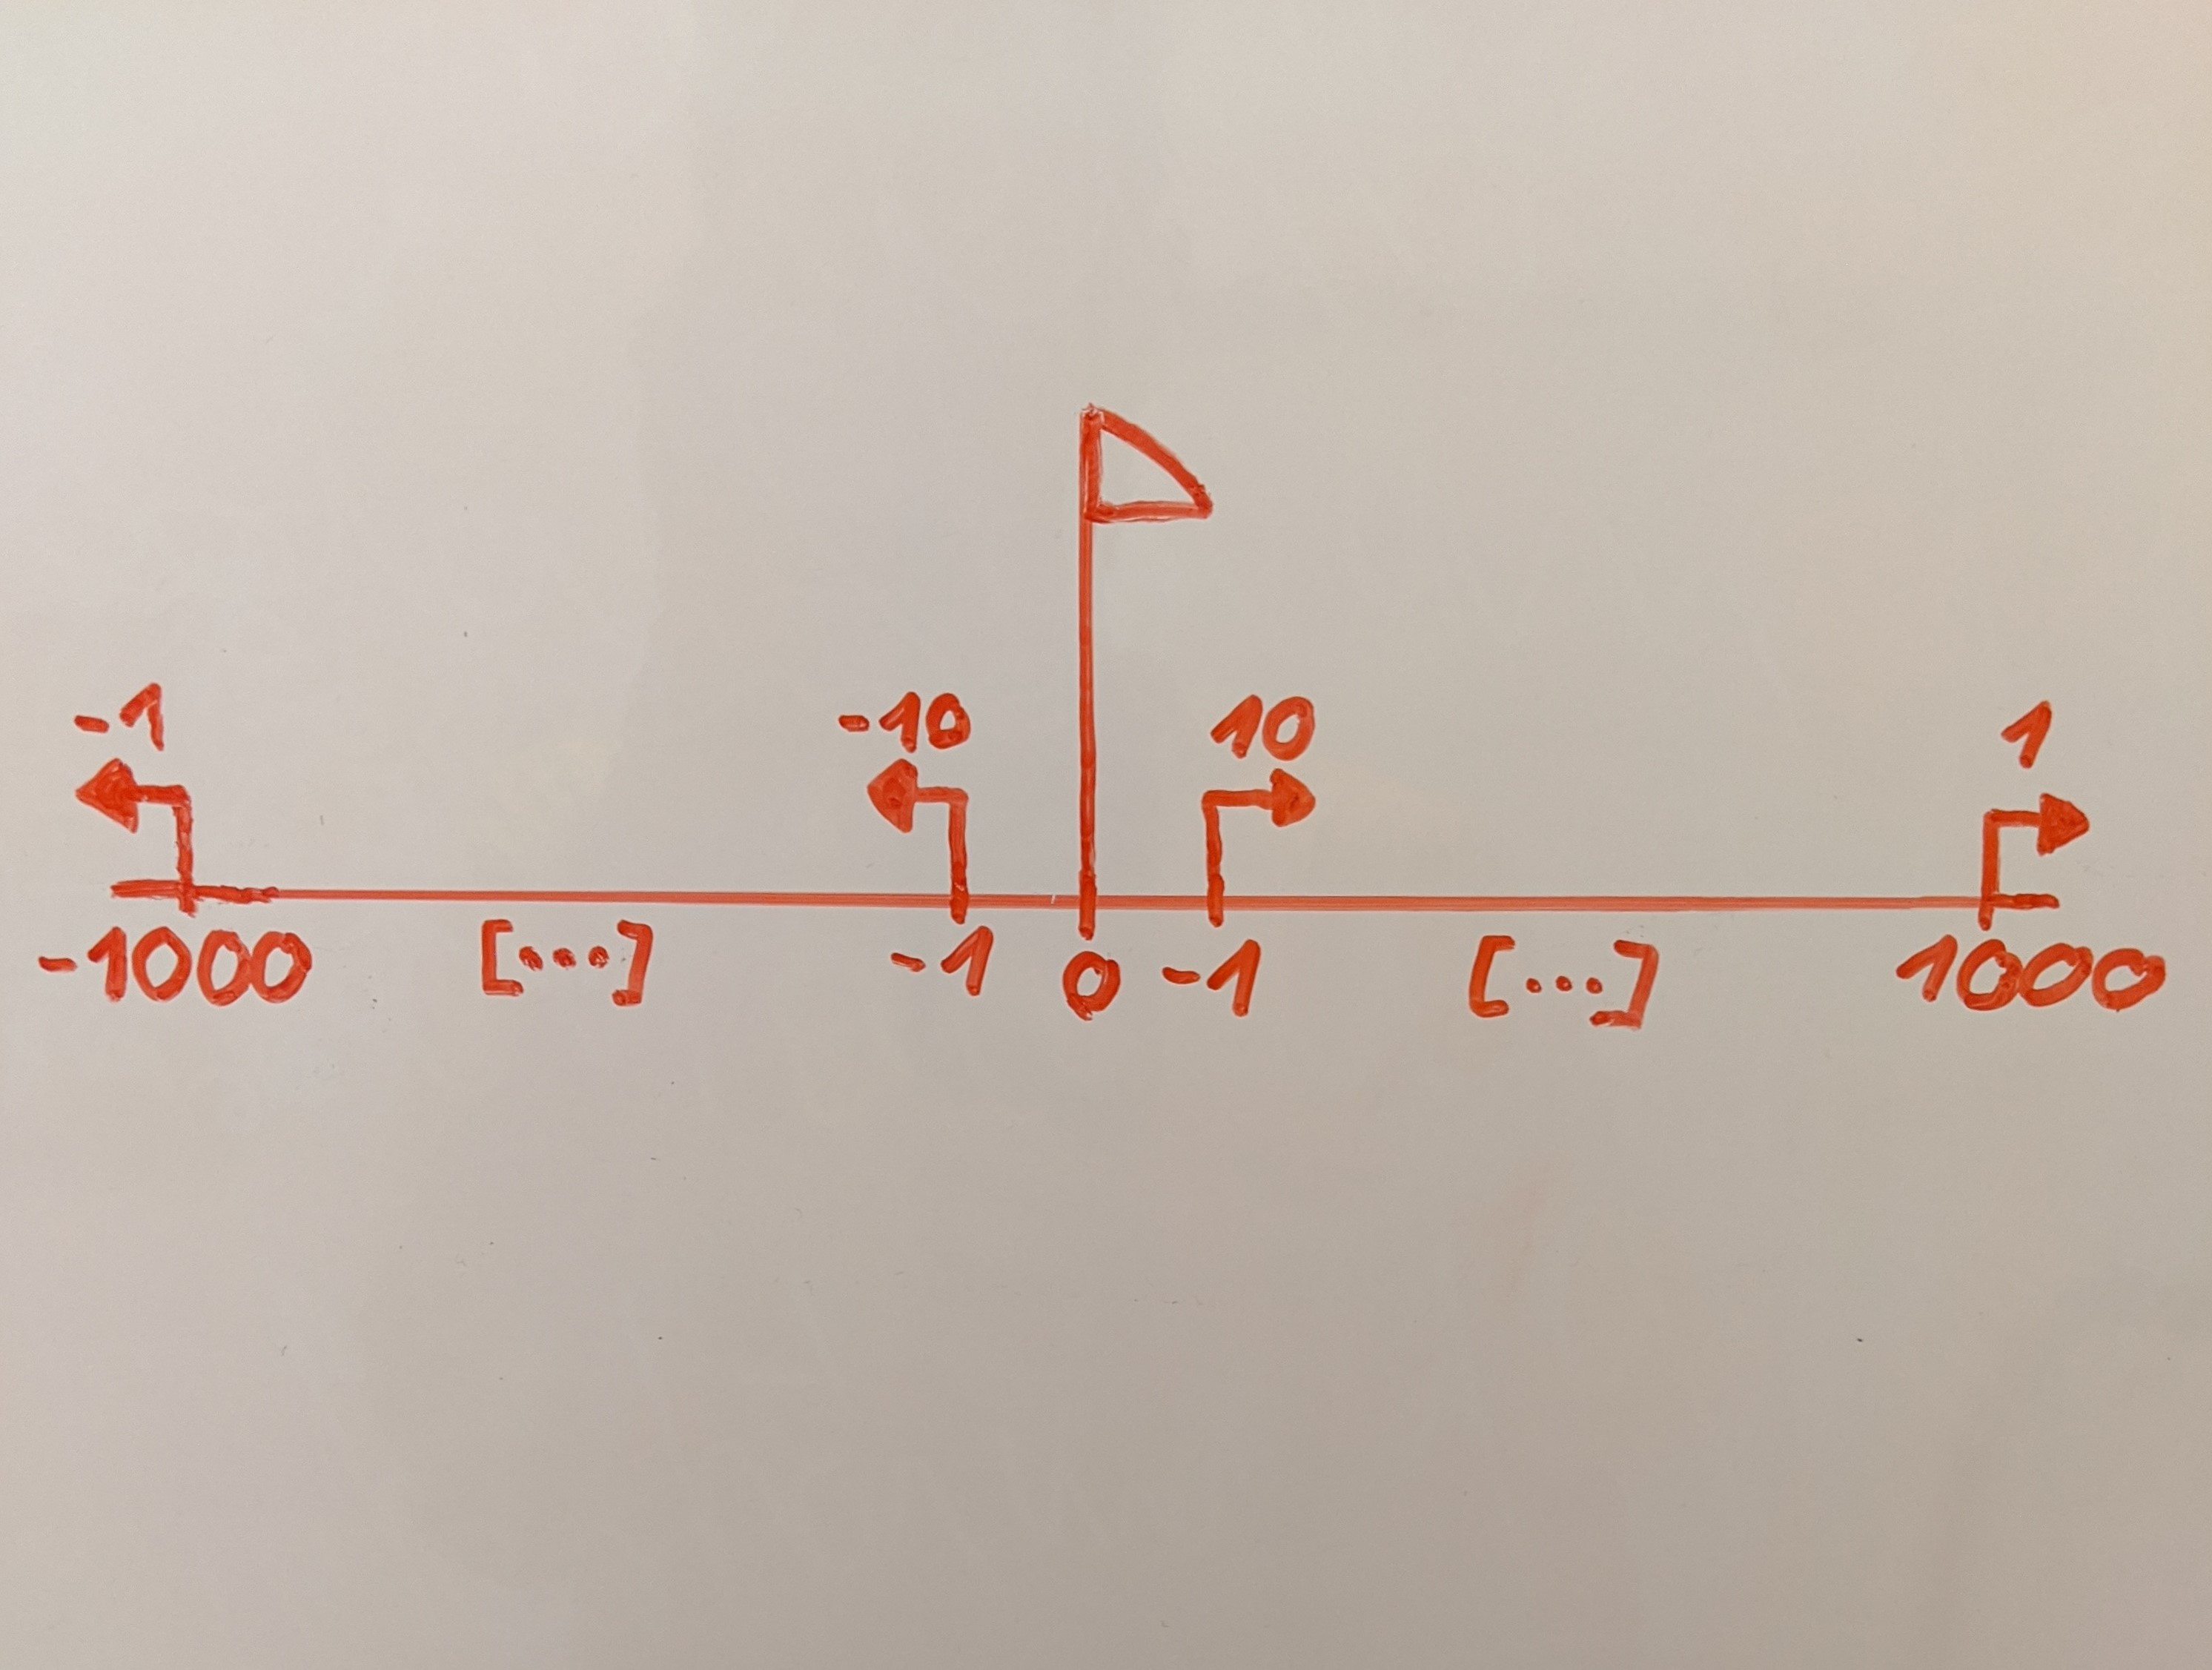
\includegraphics[scale=0.09]{../Grafiken/Whiteboard/GegenBsp1Dim.jpg}
\caption{Offensichtlich würde der Verfolger mit der Geschwindigkeit $v_{verfolger}=11$ deutlich länger für eine Tour brauchen, sofern er zunächst alle Ziele auf der einen und dann auf der anderen Seite abarbeitet. Hierbei wäre es sinnvoll, zunächst die Ziele $(-1,-10)$ und $(1,10)$ einzuholen.}
\label{fig:GegenBsp1Dim}
\end{figure}
Im worst case geht $t\rightarrow\infty$, sobald die äußersten Ziele noch deutlich weiter entfernt vom Ursprung aus liegen. 

Die Autoren aus \cite{helvig} definierten anschließend Wendepunkte und bewiesen ihre Korrektheit. Nur an diesen ist es dem Verfolger möglich, die Richtung zu ändern. Wendepunkte sind dabei die schnellsten Ziele auf der rechten bzw. rechten Seite des Verfolgers. Sofern der Verfolger vor einem Wendepunkt umkehrt, verlängert sich die Tour und ist damit nicht mehr optimal.

\begin{definition}
Ein Zustand $A$ ist definiert durch die aktuelle Position des Ziels ($s_k$), an dem sich der Verfolger zur Zeit befindet und dem schnellsten Ziel auf der gegenüberliegenden Seite des Ursprungs ($s_f$). Es ist also wieder eine Tupeldarstellung
\begin{align*}
A = (s_k, s_f)
\end{align*}
möglich, wobei $s_k$ und $s_f$ wiederum Tupel sind (siehe Definition \ref{def:Ziel}). 
\end{definition}
Ein Zustand stellt eine Momentaufnahme der Tour dar. Dabei wird ein potentieller Wendepunkt repräsentiert. Um die optimale Tour zu bestimmen, muss an jedem dieser Punkte korrekt entschieden werden, ob sich der Verfolger weiter in die Richtung bewegt oder $s_f$ auf der anderen Seite des Ursprungs verfolgt. Im Gegensatz zu den anderen Zuständen besitzen $A_0$ und $A_{final}$ keine Tupel. Dabei handelt es sich um den Start und Endzustand, welche bei jeder Tour gleich sind. Der Verfolger befindet bei beiden dieser Zuständen im Ursprung. 
Mit der Funktion $t$ wird einem Zustand die aktuell minimale Zeit zugewiesen, mit der der Zustand über andere Zustände bis dahin am schnellsten erreichbar ist (siehe Definition \ref{def:UpdatedPos}). Offensichtlich gilt demnach $t[A_0] = 0$. 

Wie bereits erwähnt, gibt es in den meisten Fällen Ziele, welche keine potentiellen Wendepunkte darstellen und somit nicht zur optimalen Tour beitragen. Um die Laufzeit und Speicherkomplexität zu reduzieren, können diese zunächst eliminiert werden. Es handelt sich dabei um Ziele, die sowieso eingeholt werden. Zunächst wird jedes Ziel in die Liste \emph{Left} oder \emph{Right} eingefügt, abhängig davon, ob sich das Ziel bei $timestamp = 0$ auf der linken oder rechten Seite des Ursprungs befindet. Anschließend werden \emph{Left} und \emph{Right} in absteigender Reihenfolge nach den Geschwindigkeiten sortiert. Ziele, welche sich nun näher am Ursprung befinden
und zugleich langsamer sind als ein anderes aus der jeweiligen Liste, werden eliminiert. Damit beinhalten \emph{Left} und \emph{Right} ausschließlich potentielle Wendepunkte. 

Um nun alle Zustände zu bestimmen, wird jede Kombination aus den Listen \emph{Left} und \emph{Right} und umgekehrt für $s_k$ und $s_f$ eingesetzt und in die Zustandsliste $States$ eingefügt. Anschließend wird $States$ in absteigender Reihenfolge nach der Summe der Indizes der Ziele aus den Listen \emph{Left} und \emph{Right} sortiert (siehe Abbildung \textcolor{red}{TODO: Bsp mit den Zielen aus der Abbildung 2.1}). Somit befinden sich die Kombinationen bzw. Zustände aus den schnellsten Zielen am Listenanfang von $States$.

\begin{definition}
Ein Zustandsübergang von Zustand A in den Zustand B wird mit
\begin{align*}
\tau = A\rightarrow B
\end{align*}
definiert. Der Übergang $\tau$ gibt dabei die Zeit $\tau$ (siehe Definition \ref{def:WegZeit}), um von dem aktuellen Zustand $A$ in den nächsten Zustand $B$ zu gelangen).
\end{definition}

Ausgehend von einem Zustand, gibt es bis zu zwei Zustandsübergänge. Dabei handelt es sich von dem nächst-schnellsten auf der linken oder rechten Seite des Ursprungs. Die Übergänge werden dann als $\tau_{left}$ und $\tau_{right}$ bezeichnet. Sofern jedes Ziel auf einer Seite eingeholt wurde, wird der Übergang $\tau_{final}$ in $A_{final}$ gewählt. Für die Berechnung von $\tau_{final}$ wird die Zeit vom aktuellen Zustand bis zum Einholen der restlichen Ziele auf der anderen Seite des Ursprungs und zusätzlich die Rückkehr zum Ursprung berechnet. Offensichtlich existiert eingehend in $A_0$ und ausgehend von $A_{final}$. 

Wie bereits erwähnt, ist die Zustandsliste $States$ nach der Summe der Indizes aus \emph{Left} und \emph{Right} in absteigender Reihenfolge sortiert. Mit zwei Möglichkeiten von $\tau_{Left}$ und $\tau_{right}$ führt jeder Zustand in einen anderen Zustand mit einem höheren Index. Dabei erhält der Startzustand $A_0$ die Summe $-1$, wodurch die Zustandsübergänge in die Zustände mit dem Summenwert von $0$ führen. Die Zustände mit der höchsten Summe führen in $A_{final}$ (Dies gilt sowieso mit der vorherigen Regelung). Mit diesen Bedingungen konnte nun aus $States$ ein Graph $G$ erzeugt werden. Anhand der Abbildung 2.3 (siehe Abbildung \textcolor{red}{TODO: Bsp mit der Abbildung 2.2}) ist diese Modellierung anhand des bisherigen Beispiels aus Abbildung 2.1 und 2.2 gut nachvollziehbar.

\begin{definition}
Ein Graph sei mit
\begin{align*}
G = (V,E)
\end{align*}
über definiert. Hierbei werden die Knoten $V$ durch die Zustände $A_i \in States$ und $E$ durch die jeweiligen Zustandsübergänge $\tau$ repräsentiert.
\end{definition}

Mit der Bedingung, dass Übergänge nur in Zustände mit höheren Summenwerten führen, ist $G$ ungerichtet und azyklisch. Man gelangt also nach spätestens $n$ Zuständen (exklusive $A_0$) in $A_{final}$. 

Mit der Modellierung des Problems als Graphen und den Eigenschaften, dass dieser azyklisch und in topologischer Reihenfolge sortiert ist, kann das Problem mit einem einfachen \emph{Kürzeste-Wege}-Algorithmus gelöst werden. Hierbei kann eine simple Heuristik, zum Beispiel \cite{brandstadt1994kurzeste}, verwendet werden, um den kürzesten Weg von $A_0$ nach $A_{final}$ zu bestimmen.

Mit der Bestimmung des kürzesten Pfades muss am Ende noch bestimmt werden, welche Ziele zwischen den Zuständen eingeholt wurden. Damit werden die anfangs eliminierten Zustände wieder der Tour hinzugefügt und bestenfalls (richtige Implementierung) ist somit die optimale Tour bestimmt.

\section{Algorithmus von Helvig, Robins and Zelikovsky}

Mit diesen Voraussetzungen haben die Autoren von \cite{helvig} einen exakten $\mathcal{O}(n^2)$-Algorithmus für eindimensionale Fälle entwickelt, welcher auf dynamischer Programmierung basiert. Dieser bestimmt dabei die optimale Tour für die Eingabeinstanz. 

Nach dem Schema aus dem vorherigen Abschnitts werden wieder die Listen \emph{Left}, \emph{Right} und $States$ generiert. Anschließend wird durch jeden der $n^2$ Zustände iteriert. Für das einfachere Verstehen des Algorithmus wurde der Graph $G$ zwar beschrieben, aber nicht generiert. Somit wird der Speicherplatz reduziert und damit die Effizienz des Algorithmus verbessert. Diese \emph{On-the-fly}-Methode, um den Graph $G$ zu generieren, ist durch die topologische Sortierung möglich. Damit ist ist für jeden Zustand sichergestellt, dass dieser mit minimaler Zeit erreicht wurde. Zudem ist nicht für jeden Zustand eine Berechnung der Übergänge in andere Zustände nötig. Einige werden ausgelassen oder führen direkt in $A_{final}$. Dies lässt sich auf das Vorgehen des Algorithmus zurückführen. Für einen Zustand $A_i$ wird dabei eines der folgenden Schritte ausgeführt:
\begin{itemize}
\item Wenn in $A_i$ keine eingehenden Übergänge besitzt, führe mit dem nächsten Zustand in der Liste fort. Dies tritt genau dann auf, wenn $t[i] = \infty$.
\item Falls der Verfolger jedes Ziel auf einer Seite des Ursprungs eingeholt hat, erzeuge einen Übergang $\tau_{final}$ in $A_{final}$. Berechne die Zeit, um die verbleibenden Ziele auf der anderen Seite einzuholen und zusätzlich die Retour zum Ursprung. 
\item Berechne ansonsten $\tau_{Left}$ und $\tau_{Right}$, welche den Verfolger entweder zum schnellsten Ziel auf der rechten oder linken Seite schickt. Falls die Zeit addiert mit dem aktuellen Zeitstempel $t[i]$ kleiner ist, als bisher von einem anderen Zustand, aktualisiere $t[A_{Left}]$ bzw. $t[A_{Right}]$ mit diesem Wert.
\end{itemize}

Schließlich werden alle (auch eliminierten) Ziele zwischen den Wendepunkten berechnet und in der richtigen Reihenfolge zusammengefügt. Somit wird eine optimale Tour durch die Kombination aus topologischer Reihenfolge und linearer Programmierung garantiert.


\section{Zwei-orthogonale-Achsen-Fall}

Zusätzlich zur Achse vom eindimensionalen Fall wird eine weitere Achse hinzugefügt, auf denen sich die Ziele und der Verfolger bewegen können. Die Achsen liegen dabei orthogonal zueinander. Den Ziele ist es dabei nicht erlaubt, an dem Schnittpunkt die Achse zu wechseln. Ein Ziel befindet sich also entweder auf der waagerechten oder senkrechten Achse. 

Mit der neuen Achse könnte für die Positionsbestimmung eine zweidimensionale Koordinate verwendet werden. Allerdings wäre einer dieser Koordinaten immer gleich $0$, da jegliche Bewegungen der Ziele und des Verfolgers auf die Achsen beschränkt sind. Somit ist nur eine einfache Ergänzung der Definition \ref{def:Ziel} um einen booleschen Wert $a$ nötig. Die Position $p_i$ wird dabei mit 
\begin{align*}
p_i = \mathbb{R} \times a | a\in \{true, false\}
\end{align*}
neu definiert. Dabei gibt $a$ die Achse an, \emph{true} steht für die waagerechte, \emph{false} für die senkrechte Achse. Die Ziele werden nun neben den Listen \emph{Left} und \emph{Right} auch in die \emph{Top} und \emph{Bottom} einsortiert. Dabei deckt \emph{Top} den positiven und \emph{Bottom} den negativen Koordinatenbereich ab. Mit dieser Ergänzung gelten weiterhin alle anderen der vorherigen Definitionen.

\section{Input $\&$ Output}

Um Heuristiken aufzustellen und zu bewerten ist ein sinnvoller und einheitlicher Input und Output notwendig. Für den Input wird eine Menge $T$ von Zielen sowie die initiale Position und Geschwindigkeit des Verfolgers erwartet. Dies reicht aus, um eine Tour zu bestimmen. 

Beim Output kommt es darauf an, wie detailliert die Tour beschrieben werden soll. Als offensichtliche Parameter werden die Tourlänge und Tourzeit zurückgegeben. Damit ist allerdings die Tour schlecht nachvollziehbar. Demnach werden die Ziele in der vom Verfolger eingeholten Reihenfolge zurückgegeben. Dabei verfügt jedes Ziel über die Position und Zeit in der der Verfolger es eingeholt hat. Um die Tour komplett nachvollziehen, ist eine graphische Anwendung sinnvoll, aber nicht notwendig. 
Die Algorithmen dieser Arbeit werden dabei einfach nur die Ziele in der eingeholten Reihenfolge zurückgeben. Je nach Implementierung kann dann einem Ziel dabei die eingeholte Zeit zugeordnet werden, womit man dann anschließend alle restlichen Informationen berechnen kann. 

Sobald allerdings eine ungültige Eingabe, z.B. wenn eine Zielgeschwindigkeit größer als die Verfolgergeschwindigkeit ist, wird eine \glqq Nein\grqq-Instanz zurückgegeben. Dies wird allerdings in den Algorithmen vorausgesetzt und nicht extra behandelt. 

\chapter{Theoretische Grundlagen für den zwei-orthogonale-Achsen-Fall}



\begin{description}
\item[Lemma 3.1]
\textcolor{red}{TODO: Lemma mit $v_{verfolger} == v_{max}$}
%\begin{align*}

%\end{align*}
\end{description}

\begin{description}
\item[Proof]
\textcolor{red}{TODO: Proof}
%\begin{align*}

%\end{align*}
\end{description}



\chapter{Heuristiken für den zwei-orthogonale-Achsen-Fall}
\begin{definition}
\textcolor{red}{TODO: Prioritätsdef.}
%\begin{align*}

%\end{align*}
\end{definition}

%\chapter{Conclusion}
\chapter{Zusammenfassung und Ausblick}
\textcolor{red}{TODO}



\begin{bibtex-entries}
@article{helvig,
  title={The moving-target traveling salesman problem},
  author={Helvig, Christopher S and Robins, Gabriel and Zelikovsky, Alex},
  journal={Journal of Algorithms},
  volume={49},
  number={1},
  pages={153--174},
  year={2003},
  publisher={Elsevier}
}

@article{moraes,
  title={Experimental Analysis of Heuristic Solutions for the Moving Target Traveling Salesman Problem Applied to a Moving Targets Monitoring System},
  author={de Moraes, Rodrigo S and de Freitas, Edison P},
  journal={Expert Systems with Applications},
  year={2019},
  publisher={Elsevier}
}

@inproceedings{hammar,
  title={Approximation results for kinetic variants of TSP},
  author={Hammar, Mikael and Nilsson, Bengt J},
  booktitle={International Colloquium on Automata, Languages, and Programming},
  pages={392--401},
  year={1999},
  organization={Springer}
}

@incollection{brandstadt1994kurzeste,
  title={K{\"u}rzeste Wege},
  author={Brandst{\"a}dt, Andreas},
  booktitle={Graphen und Algorithmen},
  pages={106--123},
  year={1994},
  publisher={Springer}
}
\end{bibtex-entries}



% If you need to have an appendix (I advise against it), insert it
% here using, first, \appendix and then \chapter and then,
% possibly, \section. 
%
% \appendix
%
% \chapter{Technical Appendix}
%
% \section{Experimental Parameters} % possibly
%
% Again, I advise against using an appendix.


\end{document}

%\begin{lemma|proof}
